\section{INTRODUCTION}

Table tennis is a game that is challenging and particularly interesting for robotics. It is possible to combine different automation, planning and movement generation schemes and study how close they come to imitating expert human behaviour. Optimality plays an important role in the improvement of striking trajectories.

\begin{figure}[t!]
\center
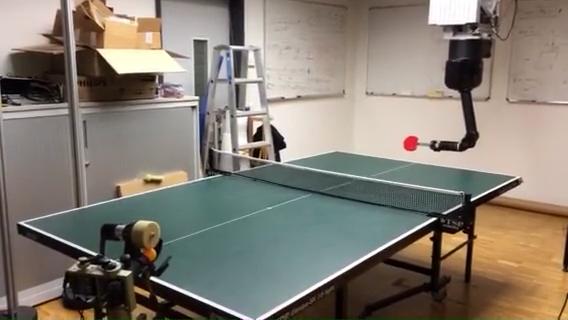
\includegraphics[scale=0.4]{robot1.png}			
\caption{Robotic table tennis setup with four cameras on the corners of the ceiling tracking the ball at 60 Hz. We filter the raw ball data provided from the cameras with an Extended Kalman Filter and predict the ball trajectory well in advance of the trajectory generation. A constrained nonlinear optimization problem is solved to find an optimal striking trajectory as well as an optimal striking time.}
\label{robot}
\end{figure}
% REPLACE PHOTO WITH ANOTHER ONE INCLUDING CAMERAS

In the rest of this paper, we describe the trajectory generation framework in detail, giving more examples and the necessary intuition where needed. In Section~\ref{relatedWork} we introduce previous work on table tennis and other relevant trajectory generation frameworks. In Section~\ref{method} we formalize robot trajectory generation as a specific optimal control problem and incorporate probabilistic modeling within this framework. In Section~\ref{alg} we discuss a two-stage optimization approach for optimizing the previously introduced cost functional. In Section~\ref{results} we evaluate the performance of this approach and compare it with previous inverse kinematics (IK) approaches. Experiments in our robotic table tennis setup are given. In the final section~\ref{end} we discuss several promising extensions on this framework. %VHP-based

\begin{figure}[t!]
\centering
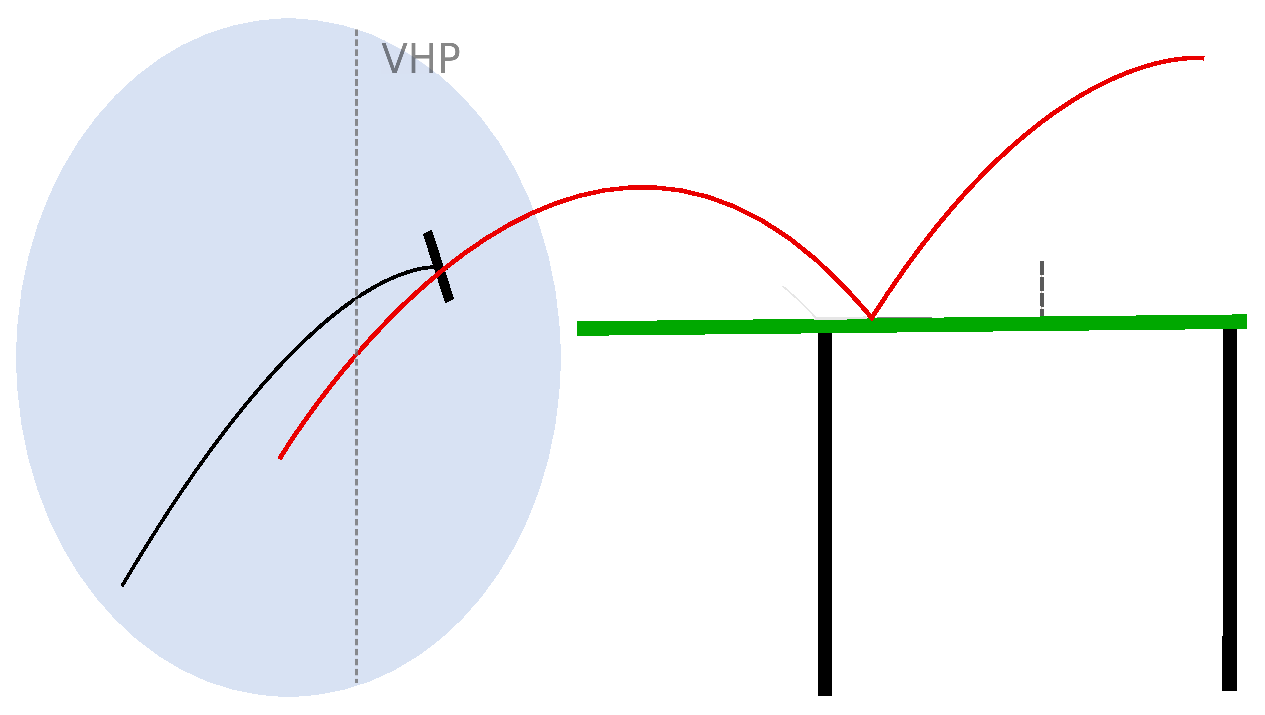
\includegraphics[scale=0.4]{drawing.eps}			
\caption{Illustrating the main idea behind this paper: fixing a virtual hitting plane (VHP) can make the generated trajectories unnecessarily restrictive and the resulting inverse kinematics may be infeasible. We instead consider the whole ball trajectory in our trajectory generation framework and optimize for the hitting time as well as the hitting point. Racket trajectory and the mean of the ball trajectory are shown in black and red, respectively. VHP is shown as a dotted gray line, the workspace of the robot is shown as an ellipsoidal light blue region.}
\label{mainIdea}
\end{figure}